\documentclass[10pt,letterpaper]{article}
\usepackage[utf8]{inputenc}
\usepackage{amsmath}
\usepackage{amsfonts}
\usepackage{amssymb}
\usepackage{graphicx}
\RequirePackage{caption}
\RequirePackage{subcaption}
\author{Christopher C. Lamb}
\title{Distributed Roots of Trust for Mobile Devices}
\begin{document}
\maketitle
\begin{abstract}
In this paper we outline a specific approach to developing software Roots of Trust that can provide a range of protection to sensitive information. This approach includes a strategy to incorporate currently unexposed hardware-based information protection as well as software-based methods that can be implemented and used today.
\end{abstract}

\section{Introduction}
Mobile computing is becoming more ingrained in everyone's day-to-day lives. Cellular telephones have become more like mobile computing platforms than simple communication devices, while tablet computing has created an entirely new style of computer access. These new computing platforms provide unprecedented access to information on demand, but are paradoxically hosted on operating systems that are much more closed than their traditional desktop predecessors. Driven by undeniable cost pressures, device vendors have been slow to adopt more secure computing practices pioneered on desktop systems. Furthermore, as a result of the closed mobile operating system ecosystem, security-minded independent software vendors have been unable to develop innovative security features via system hardware.

Implementing Roots of Trust in mobile systems to help solve these issues is problematic given the current mobile device ecosystem, in which operating systems are rigorously controlled by vendors, leading to an environment hostile to innovation. This leads to distinct challenges with technology development, in which software accessing hardware capabilities must be adopted and installed by the manufacturer or carrier, while software developed by external parties can only take advantage of application-level services and environments. Furthermore, third-party application software is precluded from taking advantage of operating system-level services unless those services are explicitly exposed to applications installed by device users.

As a group, to address these issues, we have started the development of various Roots of Trust and a Policy Engine suitable for use with mobile devices. These Roots of Trust will work together to provide secure storage, signature validation, and assertion management capabilities that will enable future integration between mobile devices and security-sensitive enterprises. The Policy Engine, using the established Roots of Trust for storage, integrity, and verification, will impose and enforce data usage policies on mobile users, providing a more secure mobile information processing environment. The Roots of Trust will be widely deployable, and will be able to take advantage of new trusted hardware features that are beginning to emerge in today's mobile systems infrastructure. The proposed systems will also be able to operate purely in software, providing levels of security near that of hardware-based solutions.

Mobile computing and other non-traditional computing paradigms are becoming more popular every day. Currently, traditional desktop and laptop systems are becoming less common as a principal computing interface for users. These systems are being replaced in all corners of the world by mobile computing devices of various profiles as primary computational tools. A commuter on the way to work in Toledo, Ohio is as likely to use global positioning on a mobile phone as a truck driver in Uganda.

This spread of mobile computing also impacts perception of preferred computing styles. In the past, organizations had strict control over the kinds of devices that could be carried into the office. Information Technology (IT) staff had absolute control over the kinds of computers employees used, and they determined if, when, and how they could access the wider Internet, as well as what kinds of computational services they could access. Today, this is no longer true. In all but the most restrictive environments, employees are able to bring telephones, tablets, or laptops into the office, whether the IT staff permits that or not. They can use ubiquitous cellular networks to attach to the global Internet, and browse whatever content they wish, unfettered by policy or technical controls.

Recognizing this trend, thought leaders have proposed allowing employees to use their own equipment to access organizational computational resources and services. This allows employees, who are accustomed to modern consumer computers that are typically years ahead of corporate resources, to use the devices they want to use, and saves organizations money that would have been spent on hardware. Though an elegant solution in some respects, this raises perhaps more thorny issues than it solves. Segregating corporate from personal data is difficult or impossible, computer security policies are legally questionable when applied to personal equipment, and data exfiltration is commonplace. 

One possible solution to this problem lies in applying trusted computing principles to mobile devices. The TCG has been working on this problem in the more traditional computing world of servers, desktops, and laptops for over a decade, and has published and implemented hardware constrained protocols and schemes to facilitate secure computer use. While reasonably successful, these approaches are difficult to apply to newer, more constrained computing devices such as phones and tablets, not to mention forthcoming watches and Google Glass. Furthermore, the business landscape for mobile devices is much different than that for traditional computing systems. Today, carriers and device manufacturers have much more control over the software installed on these smaller systems than personal computer manufacturers. Independent software houses are constrained from accessing specific hardware features by operating systems locked to devices, and are relegated to developing software within a constrained user space of the total software stack.

This leads to an innovation-stifling dilemma. Today, most mobile devices do not contain the hardware needed to functionally implement hardware-constrained trusted computing. The systems-on-a-chip that power most mobile devices are manufactured under very strict price constraints, as are the mobile devices themselves, and manufacturers are hesitant to add new hardware that would increase the costs of their products. Furthermore, both manufacturers and carriers have been hesitant to expose specific hardware functions to developers because of the additional investment in operating systems development required, along with a general hesitancy to expose security specific functions. Some newer chipsets are in fact beginning to implement more constrained secure computing capabilities that industry giants like Google have had the clout to take advantage of, but that kind of access is not provided to the developer ecosystem as a whole~\cite{Vasudevan12}.  In order to begin to provide more security on these kind of devices, enabling clean separation of enterprise from personal information, the industry needs innovative solutions providing clear ways to securely store, process, and verify information.

\subsection{Related Work}
Trusted mobile computing, especially with regard to Roots of Trust as defined by the TCG, is currently an active level of research internationally, and ARM TrustZone functionality is core to much of this work.  TrustZone enabled hardware has been used to manage and execute credentials modeled by small executable fragments~\cite{Ekberg08,Kostiainen09}.  In both these papers, the authors describe how they implement secure virtual credentials using emergent secure hardware on mobile platforms without incorporating additional hardware.  In similar work, researchers have also implemented prototypical mobile trusted platform modules~\cite{Ekberg09}.  Here the authors use currently available security extensions to implement secure computing primitives and analyze both the security posture and and possible future optimizations of their prototyped system.  Other work proposes implementing .Net Common Language Runtime features within ARM processors using TrustZone technology to take advantage of high-level computer languages already implemented within the .Net ecosystem~\cite{Santos11}.

Some initial work integrating trusted computing primitives with TrustZone-enabled hardware has yielded small successes validating this kind of approach~\cite{Winter11}.  Here, German researchers have used JSR321~\cite{JSR321} compliant software, a pending standard for Java implementing Trusted Computing primitives as defined by the TCG in a Java-centric manner, to implement a trusted platform module using TPM software from IBM~\cite{IBM-TPM}. Furthermore, the IAIK jTSS project resulted in development of Java-centric implementations of the trusted software stack ~\cite{TrustedJava}.

\section{Distributed Roots of Trust}

We envision a multi-pronged approach to providing secure Roots of Trust on mobile devices. We intend to address both the lack of support for TrustZone hardware capabilities within mobile devices in general, as well as the need for software-centric Root of Trust solutions. We will develop support within the Android Kernel for ARM\footnote{ARM is a microcontroller architecture owned by ARM Holdings, Inc.} TrustZone services, and contribute that software back to the Android Open-Source Project (AOSP) for later manufacturer or carrier handset inclusion. Simultaneously, we will develop software-only solutions that will provide secure computing functionality for older devices that are not able to take advantage of the full capabilities of today's mobile infrastructure. In this way, we will provide Roots of Trust usable on mobile platforms while hardware-based solutions are gradually being accepted and deployed in handsets and tablets by manufacturers.  Later phases of development can include implementation of Roots of Trust on other platforms; although some of these platforms use operating systems that are rigidly controlled by manufacturers and do not provide the ability for community extension~(specifically Apple's iOS operating system).

\begin{figure}
\vspace{-0.2in}
\centerline{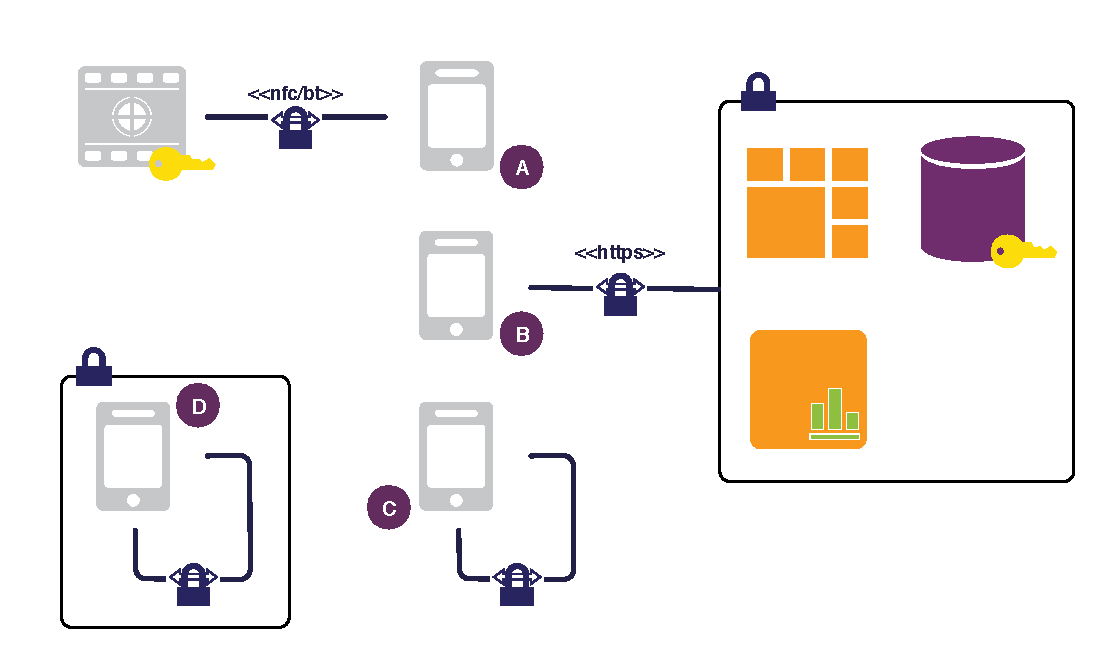
\includegraphics[width=\textwidth]{./images/conops.pdf}}
\vspace{-0.1in}
\caption{Envisioned Root of Trust configurations.}
\label{fig:conops}
\end{figure}

An overview of our approach is shown in Figure~\ref{fig:conops}.  In this figure, (A) denotes a system using Near Field Communications (NFC) or BlueTooth (BT) to communicate with an external smart card. In this scenario, keys are stored and managed on the external smartcard as much as possible, with limited exposure to the local mobile operating system. Configuration (B) represents a situation where storage root keys and other secrets are stored remotely, in a secure enclave. This is similar to option (A), but requires no new hardware to be paired with the mobile device. It does, however, require regular and predictable Internet or network access either over wireless networks or a carrier's cellular network. Configuration (C) is a pure application-level Root of Trust service. This approach has clear security vulnerabilities, in that access to keys or sensitive information is managed by the local device operating system. This is, in effect, the floor device security profile. Finally, (D) represents a device with Roots of Trust implemented with ARM TrustZone hardware support. This approach provides the most secure solution.

As much as possible, in our work we will adhere to the standards promulgated by the Trusted Computing Group (TCG)~\cite{TPMSpec}. This includes, but is not limited to, specific architectural guidance for Roots of Trust on mobile devices, software design specifications, and requirements for specific Roots of Trust including Roots of Trust for storage and measurement. Root of Trust for Measurement is not specifically identified within this call, but it nevertheless provides key trusted computing functions, and should be included within the Roots of Trust developed in the scope of this work at some time in the future via clear interface support.  We will also incorporate the appropriate security controls as identified by National Institute of Standards and Technology ( NIST)~\cite{NIST-SP-800-53} and other federal partners whenever required to further enhance the security of the developed system.

\begin{figure}
\centering
\begin{subfigure}[b]{0.45\textwidth}
\centering
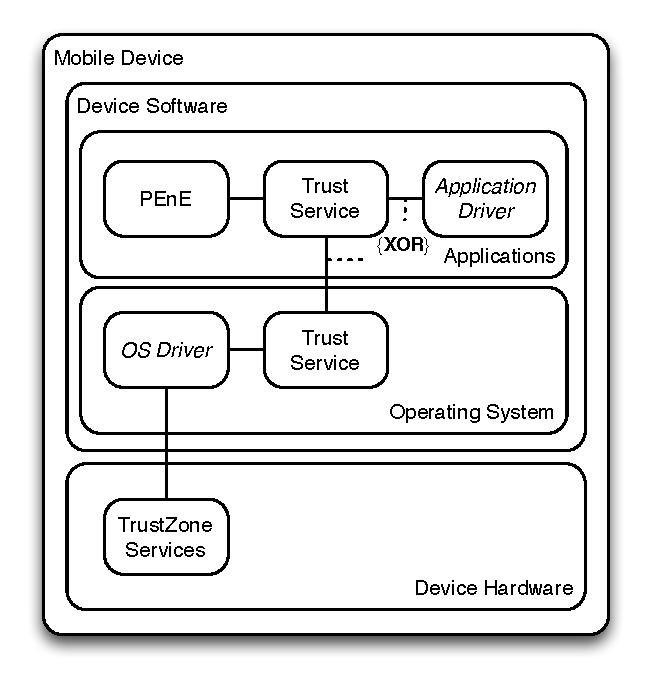
\includegraphics[width=\textwidth]{./images/hla.pdf}
\caption{Essential architecture of proposed solution.}
\label{fig:hla}
\end{subfigure}%
\begin{subfigure}[b]{0.45\textwidth}
\centering
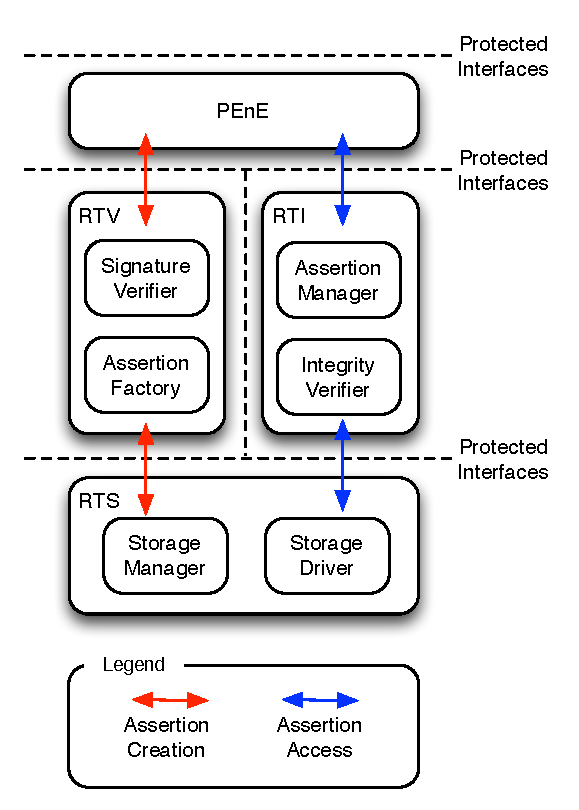
\includegraphics[width=\textwidth]{./images/layers.pdf}
\caption{Roots of Trust within Trust Service.}
\label{fig:layers}
\end{subfigure}
\caption{Architecture and Trust Service layering.}\label{fig:hla-layers}
\end{figure}

\paragraph{Clear security-centric system partitioning.}  In order to reduce the security risks associated with software-based Roots of Trust, we will clearly partition security-centric functions to reduce attack surface as much as possible. Within the Trust Service shown in Figure~\ref{fig:hla}, we will partition specific Roots of Trust and so that key storage is protected via runtime drivers using either existing hardware-based primitives via ARM TrustZone technology, remote key storage and management, or application-level drivers and security. In our proposed model, we will implement application and operating system drivers in parallel. We will contribute all operating system drivers back to the Android Open Source Project as they are developed.

One key problem we will solve in the scope of this work is mobile key storage and protection. The Trusted Computing Group outlines clear requirements with respect to how keys and secrets can be stored within a RTS. Key requirements involve how a private Storage Root Key (SRK) must be protected and used, and how other secrets can be protected within a key tree~\cite{TPMSpec}. Other specific requirements address acceptable key length and key generating algorithms~\cite{TPMSpec}. While our proposed pure application-level keystore will necessarily violate some of these requirements, our network aware and hardware-centric drivers will not. Our network aware driver will certainly impose additional overhead on some operations because of network communications; we believe it will shift security risk from the mobile device and provide an overall increase in security posture as a result.

A key feature of our proposed solution is the migration of Root of Trust functionality into the operating system via our strategy of contributions to the AOSP.  By revisiting Figure~\ref{fig:hla}, two distinct Trust Services are evident, one in the operating system and the other running in application space.  Our intention is to develop the operating system Trust Service interfaces to support operating system components appropriately.

\paragraph{Applied and attributed security metrics.} To appropriately measure and evaluate the increase in overall security posture associated with the three proposed solutions, we must identify an evaluation methodology applicable to all three domains. In the scope of this work, we propose to use a weighted combination of both attack surface and lines of exposed code associated with the trusted computing base implementing specific use and misuse cases. These cases will be described from a system perspective, easing analysis of the Root of Trust implementations. They must highlight end-to-end functionality within the Trust Service, Policy Engine, and drivers shown in Figure~\ref{fig:hla} and show where in a given set of function calls the system is most likely to be compromised. The use and misuse cases will be based on a threat model that describes the possible attackers, their motivations, and their capabilities.

\paragraph{Authenticated and authorized programming interface use.} Figure~\ref{fig:layers} shows the specific Roots of Trust implemented within the Trust Service in Figure~\ref{fig:hla}. We will not only secure and characterize the security of interfaces to specific components, but also important communication channels and sensitive information, when at motion, rest, or use.  The TCG has outlined a group of protocols to facilitate controlled access to TPM interfaces.  These protocols, specifically the Object Specific Authorization Protocol (OSAP) and Object Independent Authorization Protocol (OIAP) both rely on authorization data (AUTHDATA) maintained by an external application entity in order to prove that the entity calling into the TPM is authorized to do so.  This AUTHDATA can be related with a specific TPM owner or a system agent using a TPM, and can be unique to each agent using a TPM (a TPM will only have one owner).  This approach is well suited to implementing Roots of Trust via TrustZone technology in options C and D from Figure~\ref{fig:conops}.

\begin{figure}
\vspace{-0.2in}
\centerline{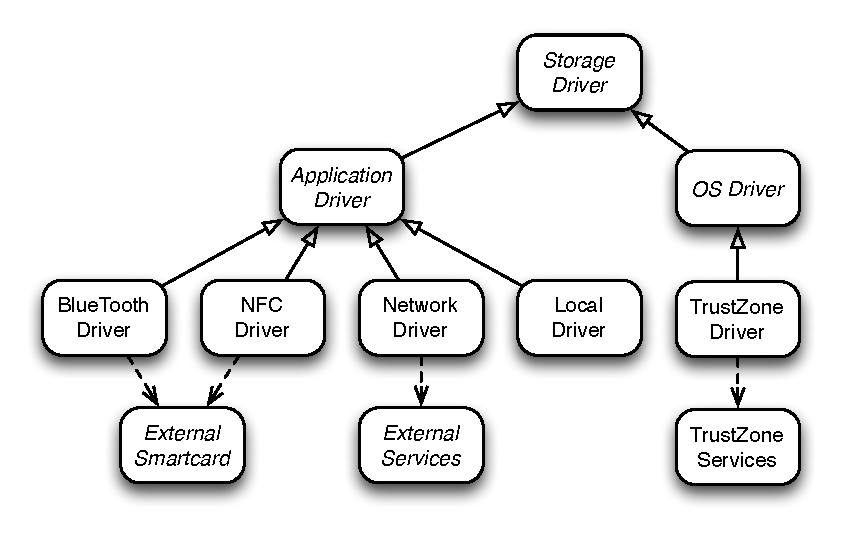
\includegraphics[width=0.65\textwidth]{./images/hierarchy.pdf}}
\vspace{-0.1in}
\caption{Driver hierarchy.}
\label{fig:hierarchy}
\end{figure}

We propose to use a similar scheme when authenticating and authorizing access to remote key stores in case B from Figure~\ref{fig:conops}.  We will use an authenticated encrypted tunnel, most likely HTTPS, over which we will pass credentials and data.  The credentials themselves will feature a rolling nonce, agent identifier, and password or passphrase, which will be hashed into a 20 byte Secure Hash Algorithm 1 (SHA1) digest.  This package will be digitally signed using an Attestation Identity Key (AIK) and then passed from the client to the server in order to authenticate the client.  The server will know the nonce used, as that nonce was set at the end of the last session or pre-installed in the mobile device when the device was first registered.  Likewise, the remote system also knows the other credentials, and can create a digest from these credentials to authenticate the mobile system.  Passwords or pass phrases can be maintained on the device, or the device can require the user to enter them when the TPM is accessed.  In the latter case, we could also one-time passwords generated from token cards like RSA SecureID cards, for example, for additional security.  Once a mobile system has authenticated, the server will authenticate itself to the mobile system using a separate rolling nonce established in the same way as the previous rolling nonce.  This nonce will be wrapped with the remote server's private key, associated with this particular mobile device.  The mobile system will receive that key, unwrap it with the public key, and compare nonces.  In both cases, the generated nonces need to be large enough and the hashing algorithm slow enough to render brute force attacks unrealistic.  Note that the remote server maintains a public/private key pair and a rolling nonce for each supported system.  Once the client and server have authenticated, the server can wrap a symmetric session key to support bulk encryption and decryption if needed for data transfer during the session.

Sensitive information must also be protected at rest when resident in the remote system.  Fortunately, the structure of a protected object hierarchy within an RTS already provides cascading encryption on contained objects, wherein parent nodes within the storage tree wrap child nodes.  The only exception to this is the private SRK, required by version 1.2 of the TPM specification to be maintained in clear text within the TPM.  We propose to store this on the remote system, but protected with a symmetric session key maintained on the mobile client, wrapped with the remote system's public key.  This session key is established at initial device registration, and reset at the end of every session.  By wrapping it with the remote system's public key, only the private key maintained by the remote system that corresponds to this specific mobile device can then access that session key and by extension the SRK.  This way, all data at rest the remote system is appropriately enciphered.  

\paragraph{Clear system state attribution.}  Common approaches used to identify system tampering involve secure hashing of protected objects using sufficiently advanced hashing algorithms using techniques like sealed memory~\cite{TPMSpec}. The TCG requires use of SHA1 as the primary hashing function for tamper detection.  In the scope of this work, we propose to investigate and implement specific system state measures within the RTV to provide evidence of tampering.  Specifically, we intend to incorporate a signed SHA1 digest of the binary representation of a software component, and optionally that component's configuration data.  The goal of this mechanism is to identify when the state of a software component has changed, and is no longer recognized to be in a known good state.  Some components may very well enable configuration changes, but in those cases, the component itself should not be altered without device owner approval.

This information would be collected by the RTV, and stored as an assertion by the RTI, within the RTS.  The Policy Engine would access the assertion via the RTI, as shown in Figure~\ref{fig:layers}.  When a change is detected in a previously stored assertion, the device owner would be notified by the Trust Service, and would indicate to the Trust Service if the new setting should be accepted and stored as a new trusted state assertion.  If so, the sensitive operation can continue and the new assertion is stored by the RTI within the RTS.  If not, the operation is canceled, and the new value discarded.  Assertions will be related to specific functions against which they assert, and will be stored as signed digests as outlined via current NIST standards~\cite{NIST-SP-800-164}.

\section{Conclusions and Future Work}

\bibliography{proposal}
\bibliographystyle{abbrv}

\end{document}